\documentclass[10pt,hyperref={bookmarks=false},aspectratio=169,usenames,dvipsnames,hideothersubsections]{beamer}

% ==================================================================
% IIIT-Delhi Beamer template
% Compile with XeLaTeX in Overleaf.
% Keep beamerthemeIIITD.sty and style1colorlarge.png in this project.
% ==================================================================

% ---------- Times-style typography ----------
\usepackage{fontspec}
\IfFontExistsTF{Times New Roman}{
  \setmainfont{Times New Roman}
  \setsansfont{Times New Roman}
}{
  % TeX Gyre Termes is a Times-compatible fallback in TeX Live.
  \setmainfont{TeXGyreTermes}
  \setsansfont{TeXGyreTermes}
}
\setmonofont{DejaVu Sans Mono}
\usefonttheme{serif}

% ---------- Packages ----------
\usepackage{array}
\usepackage{booktabs}
\usepackage{tabularx}
\usepackage{ragged2e}
\usepackage{etoolbox}
\usepackage{ifthen}
\usepackage{listings}
\usepackage{tikz}
\usetikzlibrary{positioning,arrows.meta,calc}
\usepackage{pifont}
\usepackage{hyperref}

% ---------- Colours ----------
\definecolor{codebg}{RGB}{247,248,251}
\definecolor{codeframe}{RGB}{205,211,224}
\definecolor{codeblue}{RGB}{35,82,145}
\definecolor{codegreen}{RGB}{35,115,75}
\definecolor{codered}{RGB}{160,55,55}
\definecolor{arrowcolor}{RGB}{201,216,232}
\definecolor{circlecolor}{RGB}{79,129,189}

% ---------- Listings ----------
\lstdefinestyle{CStyle}{
  language=C,
  basicstyle=\ttfamily\scriptsize,
  keywordstyle=\color{codeblue}\bfseries,
  commentstyle=\color{codegreen},
  stringstyle=\color{codered},
  numbers=left,
  numberstyle=\tiny\color{gray},
  numbersep=5pt,
  showstringspaces=false,
  breaklines=true,
  breakatwhitespace=false,
  tabsize=4,
  columns=fullflexible,
  keepspaces=true,
  frame=single,
  rulecolor=\color{codeframe},
  backgroundcolor=\color{codebg},
  xleftmargin=1.0em,
  framexleftmargin=0.65em,
  aboveskip=0.25em,
  belowskip=0.15em,
  captionpos=b
}
\lstdefinestyle{ShellStyle}{
  language=bash,
  basicstyle=\ttfamily\footnotesize,
  numbers=none,
  showstringspaces=false,
  breaklines=true,
  breakatwhitespace=false,
  columns=fullflexible,
  keepspaces=true,
  frame=single,
  rulecolor=\color{codeframe},
  backgroundcolor=\color{codebg},
  xleftmargin=0.5em,
  framexleftmargin=0.3em,
  aboveskip=0.25em,
  belowskip=0.15em
}
\lstset{style=CStyle}

% ---------- IIIT-Delhi theme and typography ----------
\usetheme[sidebarleft]{IIITD} % minimal | sidebarleft | sidebarright
\usefonttheme{serif}
\setbeamerfont{normal text}{family=\rmfamily,size=\small}
\setbeamerfont{title}{family=\rmfamily,series=\bfseries}
\setbeamerfont{subtitle}{family=\rmfamily}
\setbeamerfont{frametitle}{family=\rmfamily,series=\bfseries,size=\large}
\setbeamerfont{framesubtitle}{family=\rmfamily,size=\small}
\setbeamerfont{block title}{family=\rmfamily,series=\bfseries,size=\small}
\setbeamerfont{block body}{family=\rmfamily,size=\small}
\setbeamerfont{itemize/enumerate body}{size=\small}
\setbeamerfont{itemize/enumerate subbody}{size=\footnotesize}
\setbeamercolor{alerted text}{fg=Dandelion}
\setbeamertemplate{caption}[numbered]
\setbeamertemplate{navigation symbols}{}

% Reduce vertical crowding consistently. Long frames are also split below.
\setlength{\parskip}{2pt}
\setlength{\leftmargini}{1.35em}
\setlength{\leftmarginii}{1.2em}
\setbeamertemplate{itemize/enumerate body begin}{\setlength{\itemsep}{3pt}\setlength{\topsep}{2pt}}
\setbeamertemplate{itemize/enumerate subbody begin}{\setlength{\itemsep}{2pt}\setlength{\topsep}{1pt}}

% ---------- Section overview ----------
\newboolean{sectiontoc}
\setboolean{sectiontoc}{true}
\AtBeginSection[]{
  \ifthenelse{\boolean{sectiontoc}}{
    \begin{frame}[noframenumbering]
      \frametitle{Section Overview}
      \small
      \tableofcontents[currentsection]
    \end{frame}
  }{}
}

% ---------- Short helper commands ----------
\newcommand{\cmd}[1]{\texttt{#1}}
\newcommand{\good}{\textcolor{codegreen}{\ding{51}}}
\newcommand{\bad}{\textcolor{codered}{\ding{55}}}
\newcommand{\code}[1]{\texttt{\detokenize{#1}}}

% ---------- Presentation metadata ----------
\title[OS Lab: mmap \& madvise]{\bfseries Memory Management Aspects\\\texttt{mmap()} and \texttt{madvise()}}
\subtitle{A Linux Systems Programming Tutorial}
\author[Debarshi Roy]{Debarshi Roy\inst{1}}
\institute[IIIT-Delhi]{Operating Systems Laboratory\\Indraprastha Institute of Information Technology Delhi}
\date[OS Lab Tutorial, 4 Nov 2026]{OS Lab Tutorial Session\\4 November 2026}

\begin{document}

% ==================================================================
% TITLE AND INTRODUCTION
% ==================================================================
\frame{\titlepage}

\begin{frame}
\frametitle{Tutorial Roadmap}
\small
\begin{enumerate}
  \item Understand virtual memory, pages, and memory mappings.
  \item Learn the purpose and arguments of \code{mmap()}.
  \item Create file-backed and anonymous mappings in C.
  \item Learn how \code{madvise()} communicates expected access patterns.
  \item Compile, run, inspect, and trace the example programs.
\end{enumerate}
\vspace{0.3em}
\begin{block}{By the end of this tutorial}
You should be able to create and release a mapping, distinguish shared from private mappings, choose a suitable memory-advice value, and inspect a process's mapped regions.
\end{block}
\end{frame}

\begin{frame}
\frametitle{What We Will Practise}
\begin{columns}[T,onlytextwidth]
  \column{0.48\textwidth}
  \begin{block}{Concepts}
    \begin{itemize}
      \item Process virtual address space
      \item Pages and page faults
      \item File-backed vs. anonymous memory
      \item Shared vs. private mappings
      \item Kernel memory-use advice
    \end{itemize}
  \end{block}
  \column{0.48\textwidth}
  \begin{block}{Commands and outcomes}
    \begin{itemize}
      \item \cmd{man 2 mmap}, \cmd{man 2 madvise}
      \item \cmd{getconf PAGESIZE}
      \item \cmd{gcc} and program output
      \item \cmd{/proc/PID/maps}
      \item \cmd{strace} system-call trace
    \end{itemize}
  \end{block}
\end{columns}
\begin{alertblock}{Important}
\code{mmap()} and \code{madvise()} are C library interfaces to kernel services, not standalone shell commands. We call them from a program and use shell tools to inspect their effects.
\end{alertblock}
\end{frame}

\begin{frame}
\frametitle{A Few Terms Before We Start}
\begin{description}
  \item[Virtual address] An address used by a process; the OS and hardware translate it to a physical location.
  \item[Page] A fixed-size unit used by the virtual-memory system.
  \item[Mapping] A relationship between a process's virtual address range and a backing object or anonymous memory.
  \item[Page fault] An event raised when an access needs the OS to establish or validate a page mapping.
\end{description}
\begin{block}{Check your machine}
Run \cmd{getconf PAGESIZE}. Do not assume that every Linux machine uses the same page size.
\end{block}
\end{frame}

% ==================================================================
% SECTION 1: FUNDAMENTALS
% ==================================================================
\section{Memory Mapping Fundamentals}

\begin{frame}
\frametitle{Why Do We Need Memory Mapping?}
\begin{itemize}
  \item A process works with a \alert{virtual address space}; it does not directly choose physical RAM locations.
  \item The OS maintains mappings between virtual pages and physical page frames or backing storage.
  \item \code{mmap()} maps a file, device, or anonymous memory region into a process's virtual address space.
  \item The program accesses that region using ordinary pointer reads and writes, subject to the mapping's permissions.
\end{itemize}
\begin{block}{Typical use cases}
Large-file access, memory-mapped databases, shared-memory communication, loading executable files and libraries, and large anonymous buffers.
\end{block}
\end{frame}

\begin{frame}
\frametitle{A Simple Virtual-Memory View}
\centering
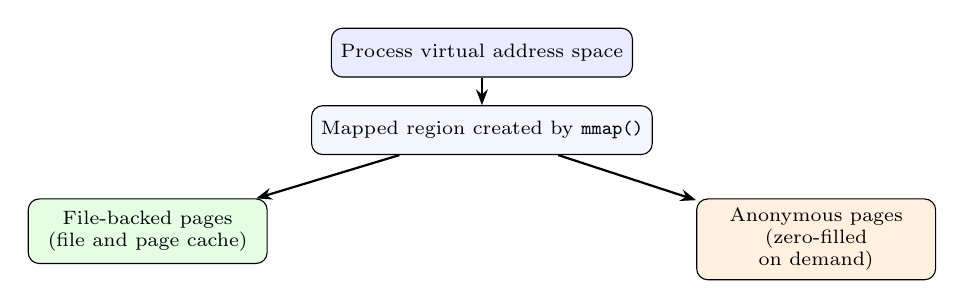
\begin{tikzpicture}[font=\scriptsize, node distance=0.35cm and 0.65cm]
  \node[draw,rounded corners,fill=blue!8,minimum width=3.1cm,minimum height=0.62cm,align=center] (proc) {Process virtual address space};
  \node[draw,rounded corners,fill=blue!4,below=0.35cm of proc,minimum width=3.1cm,minimum height=0.62cm,align=center] (map) {Mapped region created by \code{mmap()}};
  \node[draw,rounded corners,fill=green!10,below left=0.55cm and 0.55cm of map,minimum width=2.8cm,text width=2.8cm,minimum height=0.82cm,align=center] (file) {File-backed pages\\(file and page cache)};
  \node[draw,rounded corners,fill=orange!12,below right=0.55cm and 0.55cm of map,minimum width=2.8cm,text width=2.8cm,minimum height=0.82cm,align=center] (anon) {Anonymous pages\\(zero-filled on demand)};
  \draw[-{Stealth[length=2mm]},thick] (proc) -- (map);
  \draw[-{Stealth[length=2mm]},thick] (map) -- (file);
  \draw[-{Stealth[length=2mm]},thick] (map) -- (anon);
\end{tikzpicture}
\vspace{0.35em}
\begin{alertblock}{Key idea}
A mapping establishes a virtual address range. Physical pages are commonly loaded or allocated as the process accesses the range.
\end{alertblock}
\end{frame}

\begin{frame}
\frametitle{File-Backed and Anonymous Mappings}
\begin{columns}[T,onlytextwidth]
  \column{0.49\textwidth}
  \begin{block}{File-backed mapping}
    \begin{itemize}
      \item Maps bytes from an open file descriptor.
      \item Useful for large files and structured data.
      \item \code{MAP_SHARED}: writes can be visible to other mappers and are carried through to the file.
      \item \code{MAP_PRIVATE}: writes use copy-on-write and remain private.
    \end{itemize}
  \end{block}
  \column{0.49\textwidth}
  \begin{block}{Anonymous mapping}
    \begin{itemize}
      \item Has no ordinary file backing.
      \item Commonly used for process buffers and allocations.
      \item Initially reads as zero-filled memory.
      \item Typical flags: \code{MAP_PRIVATE | MAP_ANONYMOUS}.
    \end{itemize}
  \end{block}
\end{columns}
\begin{alertblock}{Remember}
Creating a mapping does not mean every page is already resident in RAM.
\end{alertblock}
\end{frame}

% ==================================================================
% SECTION 2: MMAP
% ==================================================================
\section{mmap(): Creating a Mapping}

\begin{frame}[fragile]
\frametitle{The \texttt{mmap()} Function}
\begin{block}{Header and function signature}
\begin{lstlisting}
#include <sys/mman.h>

void *mmap(void *addr, size_t length, int prot,
           int flags, int fd, off_t offset);
\end{lstlisting}
\end{block}
\small
\begin{tabularx}{\textwidth}{>{\raggedright\arraybackslash\bfseries}p{0.19\textwidth} X}
\toprule
Argument & Meaning\\
\midrule
\code{addr} & Suggested start address; normally pass \code{NULL} and let the kernel choose.\\
\code{length} & Number of bytes to map; must be greater than zero.\\
\code{prot} & Access permissions, such as read, write, execute, or none.\\
\code{flags} & Mapping type and additional options.\\
\code{fd} & Open file descriptor; use \code{-1} for an anonymous mapping.\\
\code{offset} & File offset; must be page-aligned. For an anonymous mapping, use zero.\\
\bottomrule
\end{tabularx}
\end{frame}

\begin{frame}
\frametitle{Protection and Mapping Flags}
\footnotesize
\begin{tabularx}{\textwidth}{>{\raggedright\arraybackslash}p{0.30\textwidth} X}
\toprule
\textbf{Value} & \textbf{Meaning}\\
\midrule
\code{PROT_READ} & Pages may be read.\\
\code{PROT_WRITE} & Pages may be written.\\
\code{PROT_EXEC} & Pages may be executed.\\
\code{PROT_NONE} & Pages may not be accessed.\\
\midrule
\code{MAP_SHARED} & Updates are shared with other mappings; for a file-backed mapping, updates are carried through to the file.\\
\code{MAP_PRIVATE} & Private copy-on-write mapping; writes are not propagated to the file or other mappings.\\
\code{MAP_ANONYMOUS} & No ordinary file backing; the initial contents are zero-filled.\\
\bottomrule
\end{tabularx}
\vspace{0.35em}
\begin{alertblock}{Flag selection}
Choose one of \code{MAP_SHARED} or \code{MAP_PRIVATE}. Add \code{MAP_ANONYMOUS} when no file is being mapped.
\end{alertblock}
\end{frame}

\begin{frame}[fragile]
\frametitle{First Commands: Explore the System}
\begin{lstlisting}[style=ShellStyle]
# Read the system-call documentation
man 2 mmap
man 2 madvise

# Find the page size used by this machine
getconf PAGESIZE

# Inspect the current shell's memory map
cat /proc/$$/maps | less
\end{lstlisting}
\begin{block}{What should you observe?}
\begin{itemize}
  \item The manual pages describe the arguments, flags, errors, and advice values.
  \item \code{getconf PAGESIZE} prints the page size in bytes.
  \item The final command displays the mapped regions of the current shell process.
\end{itemize}
\end{block}
\end{frame}

\begin{frame}
\frametitle{How to Read \texttt{/proc/PID/maps}}
A typical line has this structure:
\begin{center}
\code{address-range permissions offset device inode pathname}
\end{center}
\begin{itemize}
  \item \code{address-range}: start and end virtual addresses.
  \item \code{permissions}: \code{r} = read, \code{w} = write, \code{x} = execute.
  \item \code{p} = private mapping; \code{s} = shared mapping.
  \item \code{offset}: offset in the backing file, when applicable.
  \item \code{pathname}: file name for file-backed mappings; anonymous regions may have no ordinary file path.
\end{itemize}
\begin{alertblock}{Try it}
In the output of \code{cat /proc/$$/maps}, find a line with \code{rw-p} and another line with an executable permission.
\end{alertblock}
\end{frame}

\begin{frame}[fragile]
\frametitle{Example 1: Open and Size a File}
\begin{lstlisting}[language=C,basicstyle=\ttfamily\footnotesize]
int fd = open("mapped_demo.txt",
              O_RDWR | O_CREAT | O_TRUNC, 0644);
if (fd == -1) {
    perror("open");
    return EXIT_FAILURE;
}

if (ftruncate(fd, map_length) == -1) {
    perror("ftruncate");
    close(fd);
    return EXIT_FAILURE;
}
\end{lstlisting}
\begin{block}{What happened?}
The program opens the file for reading and writing, creates it if needed, truncates old contents, and sets its size to \code{map_length} bytes before mapping it.
\end{block}
\end{frame}

\begin{frame}[fragile]
\frametitle{Example 1: Create the Mapping}
\begin{lstlisting}[language=C,basicstyle=\ttfamily\footnotesize]
char *region = mmap(NULL, map_length,
                    PROT_READ | PROT_WRITE,
                    MAP_SHARED, fd, 0);

if (region == MAP_FAILED) {
    perror("mmap");
    close(fd);
    return EXIT_FAILURE;
}
\end{lstlisting}
\begin{block}{Important checks}
\begin{itemize}
  \item \code{mmap()} returns \code{MAP_FAILED} on error; do not check for \code{NULL}.
  \item The mapping is readable and writable because of \code{PROT_READ | PROT_WRITE}.
  \item \code{MAP_SHARED} makes updates visible to other mappers and carries file-backed updates through to the file.
\end{itemize}
\end{block}
\end{frame}

\begin{frame}[fragile]
\frametitle{Example 1: Write and Synchronize}
\begin{lstlisting}[language=C,basicstyle=\ttfamily\footnotesize]
const char *message = "Hello from mmap()!\n";

int written = snprintf(region, map_length, "%s", message);
if (written < 0 || (size_t) written >= map_length) {
    fprintf(stderr, "snprintf failed or message too long\n");
    munmap(region, map_length);
    close(fd);
    return EXIT_FAILURE;
}

if (msync(region, map_length, MS_SYNC) == -1)
    perror("msync");

printf("Mapped memory says: %s", region);
\end{lstlisting}
\begin{block}{Expected outcome}
The program prints \code{Hello from mmap()!}. \code{msync(MS_SYNC)} requests synchronous write-back of the mapped file range.
\end{block}
\end{frame}

\begin{frame}[fragile]
\frametitle{Example 1: Release the Resources}
\begin{lstlisting}[language=C,basicstyle=\ttfamily\footnotesize]
if (munmap(region, map_length) == -1) {
    perror("munmap");
    close(fd);
    return EXIT_FAILURE;
}

if (close(fd) == -1) {
    perror("close");
    return EXIT_FAILURE;
}
\end{lstlisting}
\begin{block}{Remember}
\code{munmap()} removes the mapped range from the process's virtual address space. Closing the file descriptor is a separate operation.
\end{block}
\end{frame}

\begin{frame}[fragile]
\frametitle{Compile, Run, and Check the File}
\begin{lstlisting}[style=ShellStyle]
# Compile with warnings enabled
gcc -std=c11 -Wall -Wextra -O0 mmap_file.c -o mmap_file

# Execute the program
./mmap_file

# Display the message stored through the mapping
head -c 19 mapped_demo.txt
printf '\n'
\end{lstlisting}
\begin{block}{Expected output}
\begin{lstlisting}[style=ShellStyle]
Mapped memory says: Hello from mmap()!
Hello from mmap()!
\end{lstlisting}
The first line is printed by the C program; the second is read back from the file.
\end{block}
\end{frame}

\begin{frame}
\frametitle{What Changes with \texttt{MAP\_PRIVATE}?}
\begin{columns}[T,onlytextwidth]
  \column{0.49\textwidth}
  \begin{block}{\code{MAP_SHARED}}
    \begin{itemize}
      \item Writes can be seen by other processes mapping the same region.
      \item File-backed updates are carried through to the file.
      \item Use \code{msync()} when explicit synchronization is required.
    \end{itemize}
  \end{block}
  \column{0.49\textwidth}
  \begin{block}{\code{MAP_PRIVATE}}
    \begin{itemize}
      \item Writes create private copy-on-write pages.
      \item Other mappers do not see those writes.
      \item The writes are not carried through to the underlying file.
    \end{itemize}
  \end{block}
\end{columns}
\begin{alertblock}{Quick experiment}
Change \code{MAP_SHARED} to \code{MAP_PRIVATE}, run the program, and inspect the file. The private writes should not change the file's contents.
\end{alertblock}
\end{frame}

\begin{frame}
\frametitle{Mapping Lifecycle}
\begin{enumerate}
  \item Open the file with access permissions compatible with the mapping.
  \item Make the file large enough for the range you will access.
  \item Call \code{mmap()} and check for \code{MAP_FAILED}.
  \item Access only addresses within the valid mapped range.
  \item Call \code{msync()} when explicit synchronization is required for a shared file mapping.
  \item Call \code{munmap()} when the mapping is no longer needed; close the file descriptor separately.
\end{enumerate}
\end{frame}

\begin{frame}
\frametitle{Common \texttt{mmap()} Pitfalls}
\small
\begin{itemize}
  \item \textbf{Wrong error check:} test against \code{MAP_FAILED}, not \code{NULL}.
  \item \textbf{Bad offset:} the file offset passed to \code{mmap()} must be page-aligned.
  \item \textbf{File too short:} accessing a mapped file page beyond the current end of the file can raise \code{SIGBUS}.
  \item \textbf{Wrong permissions:} the file descriptor's open mode must be compatible with the requested mapping and protections.
  \item \textbf{Resource leak:} release the mapping with \code{munmap()} when finished.
\end{itemize}
\begin{alertblock}{Useful distinction}
The mapping length may be any positive byte count; the file offset, not the length, is the argument that must be page-aligned on Linux.
\end{alertblock}
\end{frame}

% ==================================================================
% SECTION 3: MADVISE
% ==================================================================
\section{madvise(): Advising the Kernel}

\begin{frame}[fragile]
\frametitle{What Does \texttt{madvise()} Do?}
\begin{block}{Function signature}
\begin{lstlisting}
#include <sys/mman.h>

int madvise(void *addr, size_t length, int advice);
\end{lstlisting}
\end{block}
\begin{itemize}
  \item It tells the kernel how the application expects to use an existing memory range.
  \item The kernel may adjust read-ahead, reclaim, or page-handling decisions.
  \item Most advice values are hints, not guarantees of performance.
  \item On Linux, \code{addr} must be page-aligned; the specified length need not be page-aligned.
\end{itemize}
\begin{alertblock}{Difference in one line}
\code{mmap()} creates a mapping; \code{madvise()} gives the kernel usage advice about an existing range.
\end{alertblock}
\end{frame}

\begin{frame}
\frametitle{Common \texttt{madvise()} Advice Values}
\footnotesize
\begin{tabularx}{\textwidth}{>{\raggedright\arraybackslash}p{0.30\textwidth} X}
\toprule
\textbf{Advice} & \textbf{Application's message to the kernel}\\
\midrule
\code{MADV_NORMAL} & Use the default behavior.\\
\code{MADV_RANDOM} & Expect page references in random order; read-ahead may be less useful.\\
\code{MADV_SEQUENTIAL} & Expect sequential access; the kernel may read ahead more aggressively and reclaim pages after use.\\
\code{MADV_WILLNEED} & Expect access soon; the kernel may read some pages ahead.\\
\code{MADV_DONTNEED} & The application is finished with the range for now; the kernel may release associated resources.\\
\bottomrule
\end{tabularx}
\vspace{0.35em}
\begin{block}{Interpretation}
\code{MADV_RANDOM}, \code{MADV_SEQUENTIAL}, and \code{MADV_WILLNEED} describe expected access patterns. They do not change the program's logical data values by themselves.
\end{block}
\end{frame}

\begin{frame}[fragile]
\frametitle{Choosing an Advice Value: Code Examples}
\begin{lstlisting}[language=C,basicstyle=\ttfamily\footnotesize,numbers=none]
/* 'map' is an existing mapping of 'length' bytes. */

/* A scan from the beginning to the end of a mapped file: */
if (madvise(map, length, MADV_SEQUENTIAL) == -1)
    perror("madvise(MADV_SEQUENTIAL)");

/* A range likely to be accessed soon: */
if (madvise(map, length, MADV_WILLNEED) == -1)
    perror("madvise(MADV_WILLNEED)");

/* A workload that jumps between unrelated pages: */
if (madvise(map, length, MADV_RANDOM) == -1)
    perror("madvise(MADV_RANDOM)");
\end{lstlisting}
\begin{block}{Expected outcome}
Return value \code{0} means the advice call succeeded. It does not guarantee prefetching or a speedup; benchmark the actual workload.
\end{block}
\end{frame}

\begin{frame}
\frametitle{Understanding \texttt{MADV\_DONTNEED}}
\begin{itemize}
  \item Use it when the application no longer needs the current contents of a mapped range.
  \item It allows the kernel to discard or reclaim pages associated with that range.
  \item What a later read observes depends on the mapping type.
\end{itemize}
\begin{block}{Linux: later access after successful \code{MADV_DONTNEED}}
  \begin{itemize}
    \item \textbf{Private anonymous mapping:} pages are supplied again as zero-filled-on-demand pages.
    \item \textbf{Shared file or shared anonymous mapping:} contents are repopulated from the up-to-date backing object; the pages may not be physically freed immediately.
  \end{itemize}
\end{block}
\begin{alertblock}{Important}
\code{MADV_DONTNEED} does not mean "erase the file". Use it only when the application can safely give up the current contents of the range.
\end{alertblock}
\end{frame}

\begin{frame}[fragile]
\frametitle{Example 2: Create an Anonymous Mapping}
\begin{lstlisting}[language=C,basicstyle=\ttfamily\footnotesize]
long page_result = sysconf(_SC_PAGESIZE);
if (page_result <= 0) {
    perror("sysconf");
    return EXIT_FAILURE;
}

size_t page_size = (size_t) page_result;
size_t length = 4 * page_size;

char *mem = mmap(NULL, length, PROT_READ | PROT_WRITE,
                 MAP_PRIVATE | MAP_ANONYMOUS, -1, 0);
if (mem == MAP_FAILED) {
    perror("mmap");
    return EXIT_FAILURE;
}
\end{lstlisting}
\begin{block}{What happened?}
The program creates a private anonymous region spanning four system pages. The initial contents are zero-filled on demand.
\end{block}
\end{frame}

\begin{frame}[fragile]
\frametitle{Example 2: Write, Advise, and Read Again}
\begin{lstlisting}[language=C,basicstyle=\ttfamily\footnotesize]
for (size_t i = 0; i < 4; ++i)
    mem[i * page_size] = (char) ('A' + i);

printf("Before: %c %c %c %c\n",
       mem[0], mem[page_size],
       mem[2 * page_size], mem[3 * page_size]);

if (madvise(mem, length, MADV_DONTNEED) == -1) {
    perror("madvise");
    munmap(mem, length);
    return EXIT_FAILURE;
}
\end{lstlisting}
\begin{block}{What happens next?}
The program reads the same locations again. For this Linux private-anonymous mapping, those reads fault in zero-filled pages. The complete program is supplied as \code{madvise_demo.c}.
\end{block}
\end{frame}

\begin{frame}[fragile]
\frametitle{Example 2: Expected Output and Cleanup}
\begin{lstlisting}[language=C,basicstyle=\ttfamily\footnotesize]
printf("After : %d %d %d %d\n",
       (unsigned char) mem[0],
       (unsigned char) mem[page_size],
       (unsigned char) mem[2 * page_size],
       (unsigned char) mem[3 * page_size]);

if (munmap(mem, length) == -1) {
    perror("munmap");
    return EXIT_FAILURE;
}
\end{lstlisting}
\begin{block}{Expected output on Linux}
\begin{lstlisting}[style=ShellStyle]
Before: A B C D
After : 0 0 0 0
\end{lstlisting}
This output applies to the private anonymous mapping used in this example after a successful \code{MADV_DONTNEED} call.
\end{block}
\end{frame}

\begin{frame}[fragile]
\frametitle{Compile and Run the \texttt{madvise()} Demo}
\begin{lstlisting}[style=ShellStyle]
# Compile the complete example
gcc -std=c11 -Wall -Wextra -O0 madvise_demo.c -o madvise_demo

# Run it
./madvise_demo
\end{lstlisting}
\begin{block}{Verify the page size}
\begin{lstlisting}[style=ShellStyle]
getconf PAGESIZE
\end{lstlisting}
The C program obtains the page size at runtime using \code{sysconf(_SC_PAGESIZE)}, so it does not assume a fixed 4096-byte page.
\end{block}
\end{frame}

\begin{frame}
\frametitle{Linux-Specific Advice: Know Before Using}
\begin{itemize}
  \item \code{MADV_HUGEPAGE}: mark a range as a candidate for Transparent Huge Pages.
  \item \code{MADV_NOHUGEPAGE}: advise against Transparent Huge Pages for a range.
  \item Other Linux-specific values support cases such as memory reclaim and fork behavior.
\end{itemize}
\begin{alertblock}{Portability and kernel versions}
The available advice values and their exact behavior depend on the kernel version, configuration, and mapping type. Check \code{man 2 madvise} on the target machine before using a Linux-specific value.
\end{alertblock}
\end{frame}

% ==================================================================
% SECTION 4: HANDS-ON / DEBUGGING
% ==================================================================
\section{Hands-on Lab, Debugging, and Recap}

\begin{frame}[fragile]
\frametitle{Inspect a Process Mapping}
\begin{lstlisting}[style=ShellStyle]
# Inspect the current shell's mapping
cat /proc/$$/maps | less

# Optional summary, if procps is installed
pmap -x $$
\end{lstlisting}
\begin{block}{What to look for}
\begin{itemize}
  \item Address ranges and file offsets.
  \item Permissions such as \code{rw-p} (read/write, private) and \code{rw-s} (read/write, shared).
  \item File pathnames for file-backed mappings.
  \item Anonymous regions without ordinary file pathnames.
\end{itemize}
\end{block}
\end{frame}

\begin{frame}[fragile]
\frametitle{Trace System Calls with \texttt{strace}}
\begin{lstlisting}[style=ShellStyle]
# Trace mapping-related calls as the program runs
strace -e trace=mmap,madvise,munmap ./madvise_demo

# Save the trace for later inspection
strace -o memory_trace.txt -e trace=mmap,madvise,munmap ./madvise_demo

grep -E 'mmap|madvise|munmap' memory_trace.txt
\end{lstlisting}
\begin{block}{Expected observations}
The trace shows calls such as \code{mmap(...)} returning an address, \code{madvise(...)} returning \code{0} on success, and \code{munmap(...)} releasing a region. Runtime libraries may also create mappings.
\end{block}
\begin{alertblock}{Permissions}
Tracing a program started by \code{strace} usually does not require \code{sudo}. A lab server's security policy may still restrict tracing.
\end{alertblock}
\end{frame}

\begin{frame}
\frametitle{Common Errors: Mapping and File Access}
\small
\begin{tabularx}{\textwidth}{>{\raggedright\arraybackslash\bfseries}p{0.34\textwidth} X}
\toprule
Symptom & Check or correction\\
\midrule
\code{mmap()} returns \code{MAP_FAILED} & Check \code{errno} with \code{perror()}; verify the file descriptor, protections, flags, length, and offset.\\
\code{SIGBUS} while accessing a mapped file & Ensure the accessed file offset is within the current file size; do not truncate the file while relying on pages beyond its new end.\\
Changes do not appear in the file & Check whether the mapping is \code{MAP_SHARED}; writes through \code{MAP_PRIVATE} are copy-on-write.\\
Mapping remains after use & Call \code{munmap(addr, length)} when finished.\\
\bottomrule
\end{tabularx}
\end{frame}

\begin{frame}
\frametitle{Common Errors: Memory Advice}
\begin{itemize}
  \item \textbf{\code{madvise()} returns \code{-1}:} inspect \code{errno}; check that the address is page-aligned, the range is mapped, and the advice is supported.
  \item \textbf{Advice appears to do nothing:} most values are hints, not promises of a measurable performance improvement.
  \item \textbf{Unexpected data after \code{MADV_DONTNEED}:} check the mapping type; the follow-up behavior differs for private anonymous and shared mappings.
  \item \textbf{Tracing is denied:} check whether the server restricts \code{ptrace}; do not attempt to bypass the administrator's policy.
\end{itemize}
\end{frame}

\begin{frame}
\frametitle{Guided Tutorial Exercise}
\small
\begin{enumerate}
  \item Run the file-backed example with \code{MAP_SHARED}; change the string and verify the file.
  \item Change the flag to \code{MAP_PRIVATE}; repeat the test and compare the file.
  \item Create a \code{MAP_PRIVATE | MAP_ANONYMOUS} region and inspect its initial bytes.
  \item Apply \code{MADV_SEQUENTIAL} to a sequential file scan.
  \item Apply \code{MADV_DONTNEED} to the private anonymous mapping and inspect the next reads.
  \item Use \code{strace} to identify the mapping, advice, and unmapping calls.
\end{enumerate}
\begin{block}{Expected learning outcomes}
Explain which updates reach the file, what a later read observes after \code{MADV_DONTNEED}, and how Linux exposes a process's mapped regions.
\end{block}
\end{frame}

\begin{frame}
\frametitle{Recap: Five Things to Remember}
\begin{enumerate}
  \item \code{mmap()} creates a region in a process's virtual address space.
  \item \code{MAP_SHARED} shares updates; \code{MAP_PRIVATE} uses copy-on-write.
  \item \code{MAP_ANONYMOUS} creates memory without ordinary file backing.
  \item \code{madvise()} communicates expected usage; most advice values are hints.
  \item \code{MADV_DONTNEED} has mapping-dependent follow-up behavior.
\end{enumerate}
\begin{alertblock}{Final check}
Can you explain the difference between mapping memory, advising the kernel, and unmapping memory?
\end{alertblock}
\end{frame}

\begin{frame}
\frametitle{References and Further Reading}
\footnotesize
\begin{itemize}
  \item Linux man-pages: \href{https://man7.org/linux/man-pages/man2/mmap.2.html}{\code{mmap(2)}}.
  \item Linux man-pages: \href{https://man7.org/linux/man-pages/man2/madvise.2.html}{\code{madvise(2)}}.
  \item Linux man-pages: \href{https://man7.org/linux/man-pages/man2/msync.2.html}{\code{msync(2)}}.
  \item Linux man-pages: \href{https://man7.org/linux/man-pages/man5/proc_pid_maps.5.html}{\code{proc_pid_maps(5)}}.
  \item Linux man-pages: \href{https://man7.org/linux/man-pages/man1/strace.1.html}{\code{strace(1)}}.
\end{itemize}
\vspace{0.5em}
\centering
\Large Questions?
\end{frame}

\end{document}
